% C13 — Sewn-plank ship of Hormos (I-7). Book: vol-1/ch-07 ¶¶ "Down at the ships" and "Have a look inside", Notes [20]–[21] ([@yc, 1.19]).
% Visual comparandum for Gulf ships: BnF Arabe 5847, fol. 119v (1237, Cue C7); construction details in this cutaway follow Polo's text only (S22-E2).
\path (0,0) -- (11.43,0);
\node[dg-head] at (0,0.25) {The stitched horse-ship of Hormos, as the Book describes it};
\node[anchor=north west, inner sep=0pt] at (1.11,0.55) {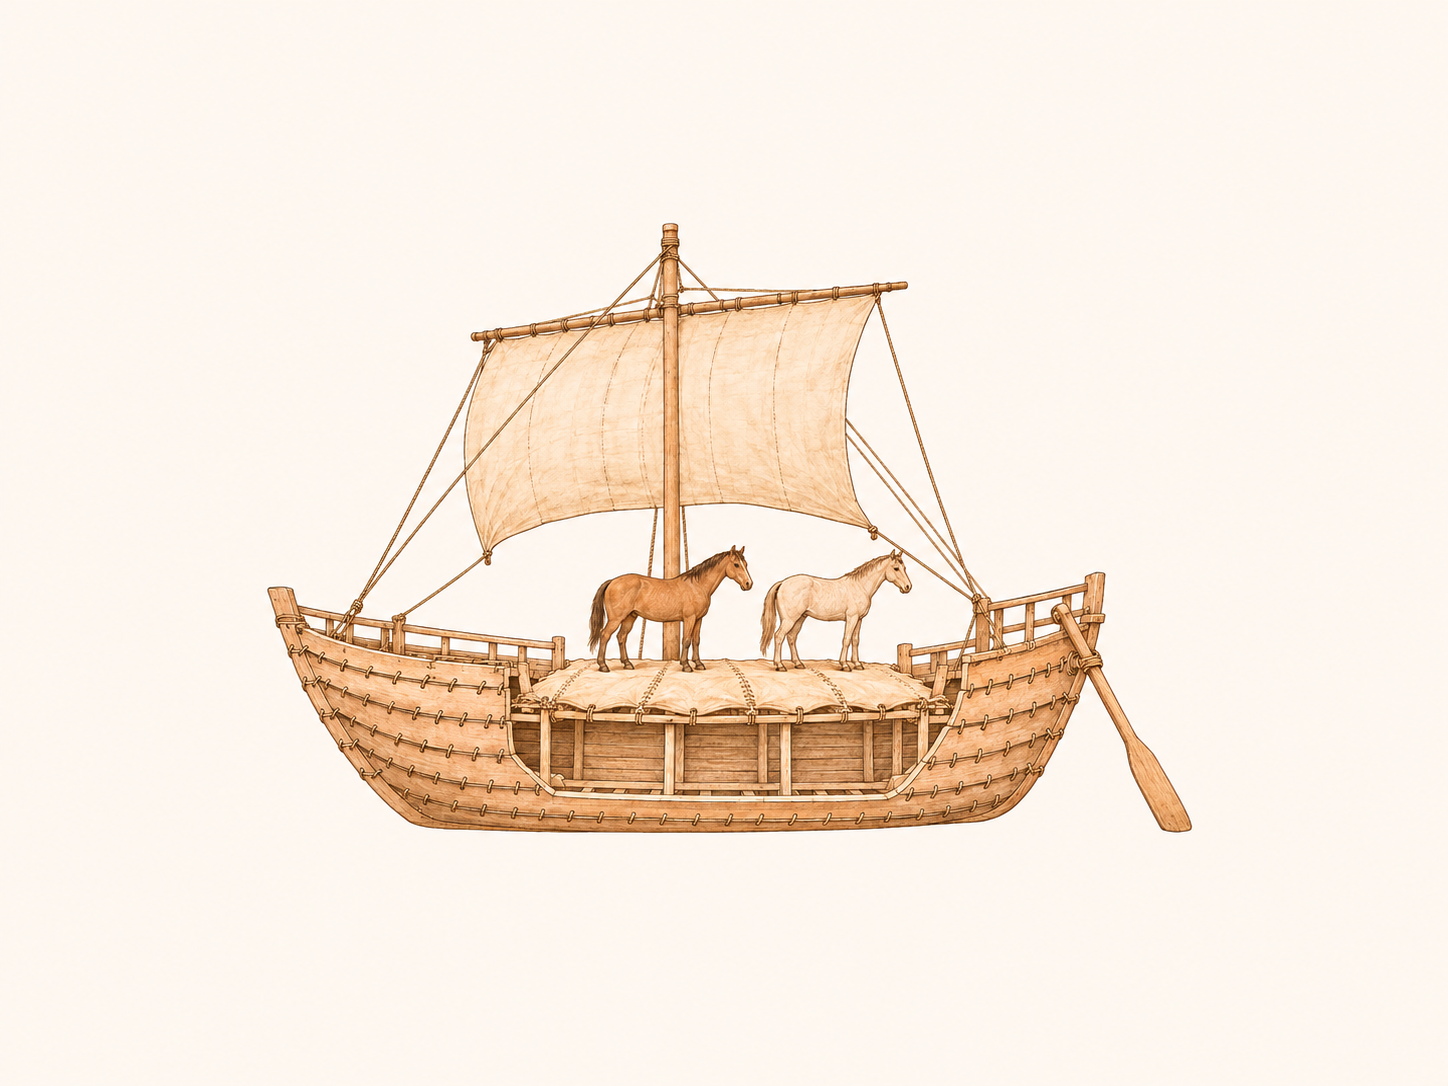
\includegraphics[width=9.20cm]{../../../manuscript/assets/plates/C13-sewn-plank-hormos.png}};
% Callouts
\draw[tl-leader] (5.35,2.75) -- (2.85,1.50);
\node[dg-text, text width=2.75cm, font=\scriptsize, anchor=north west] at (0.0,1.25) {\textbf{One mast, one sail}: Polo notes a single mast and sail};
\draw[tl-leader] (5.40,4.15) -- (8.65,2.10);
\node[dg-text, text width=2.75cm, font=\scriptsize, anchor=north west] at (8.65,1.75) {\textbf{Horses for India} stand above the hide-covered cargo};
\draw[tl-leader] (5.35,4.65) -- (2.85,3.70);
\node[dg-text, text width=2.75cm, font=\scriptsize, anchor=north west] at (0.0,3.45) {\textbf{No fixed deck}: hides spread over the cargo bales below};
\draw[tl-leader] (8.10,4.85) -- (8.65,4.15);
\node[dg-text, text width=2.75cm, font=\scriptsize, anchor=north west] at (8.65,3.95) {\textbf{One rudder} (drawn here as a quarter steering oar)};
\draw[tl-leader] (3.65,5.15) -- (3.20,6.65);
\node[dg-text, text width=5.6cm, font=\scriptsize, anchor=north west] at (0.0,6.70) {\textbf{Coir-stitched planking}: coconut-husk cord and wooden pins, with no iron nails; smeared with fish oil instead of pitch};
\node[dg-note, text width=11.2cm] at (0,7.70) {Hypothetical schematic from Polo's text. Regional finds attest sewn construction. The hull shape, lacing pattern and framing shown here are conjectural.};
